\documentclass[a4paper,12pt]{extarticle}
\usepackage[table,xcdraw]{xcolor}
\usepackage{pgfplots}
\usepackage[unicode, pdftex]{hyperref}
\usepackage[T2A]{fontenc}
\usepackage[utf8]{inputenc}
\usepackage[english,russian]{babel}
\usepackage{amsmath,amsfonts,amsthm, mathtools}
\usepackage{amssymb}
\usepackage{dsfont}
\usepackage{graphicx}
\graphicspath{{images/}}
\usepackage{wrapfig}
\usepackage{floatrow}
\usepackage{setspace}
\usepackage[headings]{fancyhdr}
\usepackage[margin=10pt,font={small,stretch=0,9},labelfont=bf,labelsep=period,
justification=centerlast]{caption}
\usepackage{array,tabularx,tabulary,booktabs}
\RequirePackage{multirow}
\RequirePackage{multicol}
\RequirePackage{longtable}
\usepackage{indentfirst}
\usepackage{hyperref}
\usepackage{icomma}
\newcommand*{\hm}[1]{#1\nobreak\discretionary{}
	{\hbox{$\mathsurround=0pt #1$}}{}}
\usepackage{soulutf8} 
\usepackage{etoolbox} 
\usepackage{geometry}
\geometry{top=20mm}
\geometry{bottom=20mm}
\geometry{left=20mm}
\geometry{right=20mm}
\DeclareMathOperator{\sgn}{\mathop{sgn}}
\usepackage[OT1]{fontenc}
\usepackage{amsmath}
\usepackage{amsfonts}
\usepackage{amssymb}
\usepackage{wasysym}
\usepackage{wrapfig}
\usepackage{physics}
\usepackage[normalem]{ulem}
\graphicspath{{pictures/}}
\DeclareGraphicsExtensions{.png,.jpg,.jpeg}
\usepackage{indentfirst}
\usepackage[T2A]{fontenc}
\usepackage{subfigure}
\usepackage{fancyhdr}
\usepackage{caption}

\usepackage{tabularx}
\usepackage{floatrow}
\usepackage{multicol}
\usepackage{lastpage}

\pgfplotsset{
  MyStyle1/.style={
    axis lines = middle,
    enlargelimits = true,
    grid=both,
    grid style={line width=.1pt, draw=gray!10},
    major grid style={line width=.2pt,draw=gray!50},
    minor tick num=5,
    enlargelimits=0.05,
    ticklabel style={font=\tiny,fill=white},
    xlabel style={at={(ticklabel* cs:1)},anchor=north west},
    ylabel style={at={(ticklabel* cs:1)},anchor=south east},
  }
}
\def\Slope{1.5}
\def\Intercept{-20}


% Настройка отчёркиваний и нумерации
\usepackage{fancyhdr}
\pagestyle{fancy}
\fancyhf{}

\fancyhead[L]{\nouppercase{\leftmark\hfill}}
\fancyfoot[RO, RE]{Страница \thepage \ из \pageref{LastPage}}
\renewcommand{\headrulewidth}{0.5pt}
\renewcommand{\footrulewidth}{0.5pt}

\usepackage{titlesec}
\titlelabel{\thetitle.\quad}

\pgfplotsset{compat=1.18}
\begin{document}

\thispagestyle{empty}
\begin{center}
	\textit{Федеральное государственное автономное образовательное\\ учреждение высшего образования }
	
	\vspace{0.5ex}
	
	\textbf{«Московский физико-технический институт\\ (национальный исследовательский университет)»}
\end{center}

\vspace{10ex}
\begin{figure}[!h]
  \begin{center}
    
\includegraphics[width = 0.8\textwidth]{MIPT.png}
  \end{center}
\end{figure}

\begin{center}
	
	\textbf{Лабораторная работа № 4.3.1}
	
	\vspace{1ex}
	
	по курсу общей физики
	
	на тему:
	
	\textbf{\textit{<<Изучение дифракции света>>}}
	
	\vspace{20ex}
	
	\begin{flushright}
		\noindent
		\textit{Работу выполнил:}\\  
		\textit{Легких Никита \\(группа Б05-301)}
	\end{flushright}
	\vfill
	Долгопрудный \\ \today
	\setcounter{page}{1}
\end{center}
\newpage

% Конец шаблона
\newpage

\textbf{Цель работы:} исследовать явления дифракции Френеля и Фраунгофера на одной и двух
щелях, изучить влияние дифракции на разрешающую способность оптических инструментов;
проверить теоретические соотношения для положения максимумов при дифракции Френеля
и Фраунгофера.

\textbf{В работе используются:} оптическая скамья, ртутная лампа, светофильтр, щели с регулируемой шириной, рамка с вертикальной нитью, экран с двойной щелью, микроскоп (в моем случае без микрометрического винта), зрительная труба.

\section{Дифракция Френеля}
\section*{Установка + Теоретическая справка}
\begin{figure}[h]
\centering
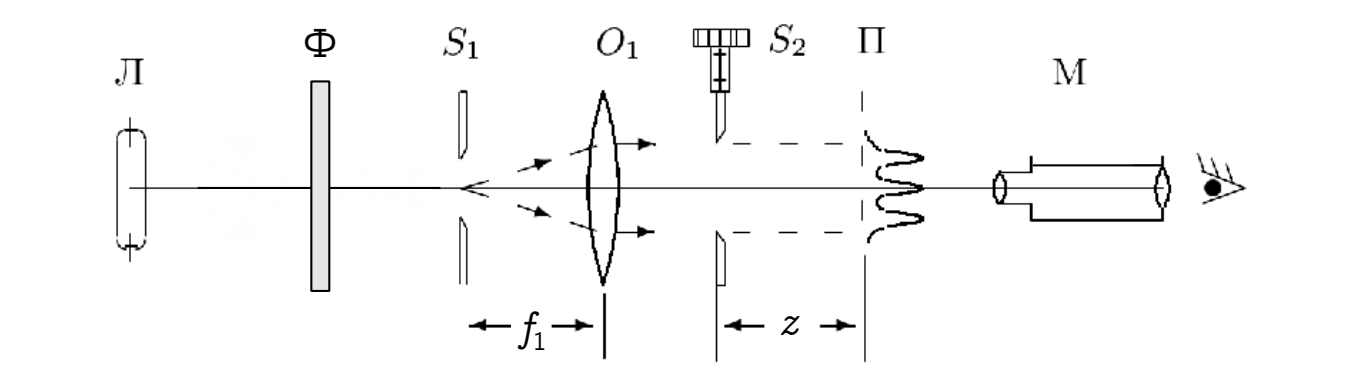
\includegraphics[width=0.9\linewidth]{pics/ustanovka_1}
\caption{Установка 1}
\label{fig:ust-1}
\end{figure}
Схема установки для наблюдения дифракции Френеля представлена на рис. 1. свет от ртутной ртутной ламы Л, пропущенный через оранжевый светофильтр Ф со средней длиной волны $\lambda$ = 578 нм, падает на входную щель $S_1$. Щель $S_1$ находится в фокусе \textit{коллиматора} — собирающей линзы $O_1$. Коллиматор создаёт параллельный пучок монохроматического света, освещающий щель $S_2$, на которой и происходит дифракция. Дифракционная картина рассматривается с помощью микроскопа М, сфокусированного на
некоторую плоскость наблюдения П.

Распределение интенсивности света в плоскости наблюдения П проще всего рассчитывать с помощью \textit{зон Френеля} \textit{(Шустера)}  Результирующая амплитуда в точке наблюдения определяется суперпозицией колебаний от тех зон Френеля, которые не перекрыты створками щели. Границы зон Френеля/Шустера $\xi_m$ определяется соотношением
\begin{equation}
    \xi_m = \pm \sqrt{mz\lambda}, m \in \mathds{N}
\end{equation}
где $\xi$ отсчитывается от центра щели, $z$ - расстояние от щели до плоскости наблюдения П, а $\lambda$ - длина волны. При ширине щели $b$ $(-b/2 < \xi < b/2)$ полное число открытых зон для
точки наблюдения на оси равно
\begin{equation}
    m_{max} = \frac{b^2}{4 \lambda z}
\end{equation}
\begin{wrapfigure}{l}{0.4\textwidth}
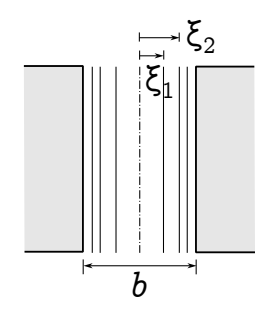
\includegraphics[width=0.39\textwidth]{pics/zones_gap.png}
\label{}
\end{wrapfigure}
Зафиксируем размер щели $b$ и проанализируем, как меняется картина в зависимости от расстояния до плоскости наблюдения $z$. Если
число открытых зон Френеля велико, $m \gg 1 (z \rightarrow 0)$, мы приходим к пределу геометрической оптики. В нём дифракционная картина отсутствует, а размер изображения щели совпадает с шириной самой щели $b$. Дифракционная картина наблюдается только в узкой полосе вблизи границ щели («дифракция на краю экрана»). При удалении от плоскости геометрического изображения эти две группы полос постепенно расширяются, заполняя всё изображение щели. При $m \sim 1$ на щели наблюдается сложная картина из небольшого числа дифракционных полос. При дальнейшем удалении $(m \ll 1, z \rightarrow \infty)$ дифракционная картина начинает упрощаться и расширяться, переходя в \textit{режим Фраунгофера} — затухающие по интенсивности эквидистантные полосы с характерным угловым размером центральной полосы $\lambda/b$. Но об этом в следующем пункте.

\section*{Задание}
\textbf{1)} Настраиваем зрительную трубу выйдя в коридор и настраивая ее на дальнее окно. (\underline{не путаем зрительную трубу с микроскопом!!})

\textbf{2)} Опреляем нуль микрометрического винта на щели, для этого проводим серию экспериментов, где мы наблюдаем момент открытия щель на фоне лампы (не смотря на сам винт) и получаем следующую серию измерений: 
\begin{tabular}{|c|c|c|c|c|c|}
\hline
$n$    & 1   & 2   & 3   & 4   & 5   \\ \hline
$b_0$, мкм & 335 & 375 & 340 & 342 & 333 \\ \hline
\end{tabular}

Получаем что $b_0 = (345\pm15)$ мкм, считаю оценку справедливой вследствие люфта винта. В дальнейшем я сразу буду вычитать $b_0$ и учитывать погрешность этого действия.

\textbf{3)-5)} Собираем схему с рис. \ref{fig:ust-1}, ловя баланс между ярокстью и контрастностью, выставляя $b \approx 0.05$ мм.

\textbf{6)-9)} Измеряя количество видимых темных полос от смещения от "четкого" положения получаем следующее: \\
\begin{tabular}{|c|c|c|c|c|c|c|}
\hline
$n$ & 1   & 2   & 3   & 4   & 5   & 6   \\ \hline
$z$, см & 2.7 & 2.3 & 1.7 & 1.2 & 0.9 & 0.8 \\ \hline
\end{tabular}

$z_0 = 52.3$ см, ширину щели же измеряем двумя способами: 1) с помощью окулярной шкалы микроскопа, там получаем $b_{\text{микроскоп}} = (0.0304\pm0.0008)$ мм $\leftarrow$ погрешность оценена как приборная + измерительная; 2) по микрометрическому винту: $b_{\text{винт}} = (0.0375\pm0.0015)$ мм $\leftarrow$ погрешность оценил как погрешность определения нуля ракрытия щели. Получили отличие в $\frac{375-304}{375+304} \cdot 2 = 0.2 = 20\%$ - достаточно большое отклонение, как по мне связано с люфтом винта и неточным совмещением предметной плоскости.

\textbf{11)} К сожалению из-за отсутствия микрометрического винта на микроскопе, получить хорошую картину не вышло, но качественно пронаблюдать получаемый эффект вышло.

\textbf{12)} Было получено что при увеличении ширины щели увеличивается плотность полос около края.

\textbf{14)} Известно что $m = n + 1$ - число открытых зон Френеля, а из формулы (1) можно выразить значение $\xi^2_m$, оценив его примерно равным $b$, строим график линеаризованной (из ф-лы (2)) зависимости: 

\begin{minipage}{0.45\textwidth}
      \begin{tikzpicture}
        \begin{axis}[
          width=1\textwidth,
          height=,
          xlabel={$m$},
          ylabel={$1/z$},
          MyStyle1,
          ]
          \draw[blue, domain=0:100] plot (\x,0.19065714285714286
*\x-0.0934571428571429);
          \addplot[purple, only marks] plot [error bars/.cd,
                x dir=both, x fixed = 0.05,
                y dir=both, y explicit,
                      ] table [
                      x=m, y=1z,
                x error minus=merr, x error plus=merr, y error minus=1zerr, y error plus=1zerr, col sep=comma] {m(z^-1).csv};
        \end{axis}
      \end{tikzpicture}
\end{minipage}
\begin{minipage}{0.45\textwidth}
    \begin{tikzpicture}
        \begin{axis}[
          width=1\textwidth,
          height=,
          xlabel={$m$},
          ylabel={$2\xi_m$, мкм},
          MyStyle1,
          ]
          \draw[blue, domain=0:100] plot (\x,370);
          \addplot[purple, only marks] plot [error bars/.cd,
                x dir=both, x fixed = 0.05,
                y dir=both, y explicit,
                      ] table [
                      x=m, y=2xi,
                y error minus=sigma2xi, y error plus=sigma2xi, col sep=comma] {xi^2.csv};
        \end{axis}
      \end{tikzpicture}
\end{minipage}

Видно что наибольшая ошибка линеаризации появляется из-за невозможности взятия $2\xi = const$, плюс есть проблема с тем, что погрешность определения нужного момента появления черных полос, оказывается соразмерным шагу между появлениями этих минимумов и это тоже дает немалые погрешнсти. Из правого графика видно что невозможно найти даже такое значение, чтобы оно попадало во все ворота значений. Из графика можно рассчитать как раз подходящее значение $\alpha = \frac{b^2}{4\lambda} \Rightarrow b = \sqrt{4\lambda\alpha} = 373$ мкм, погрешность оцениваем по формуле: $\mathcal{E}_b = \mathcal{E}_{\alpha}/2 = 4\% \Rightarrow b = (373\pm15)$ мкм. (с учетом всех ворот значений мы попали нашим значением)

Таблица значений рассчетов: 
\begin{tabular}{|c|c|c|c|c|c|}
\hline
$n$ & $m$ & $x$, см & $z$, см & $2\xi_m$, мкм & $\mathcal{E}_{2\xi_m}$, мкм \\ \hline
1 & 2 & 51.2 & 2.7  & 353        & 13       \\ \hline
2 & 3 & 50.8 & 2.3  & 399        & 17       \\ \hline
3 & 4 & 50.2 & 1.7  & 397        & 23       \\ \hline
4 & 5 & 49.7 & 1.2  & 372        & 31       \\ \hline
5 & 6 & 49.4 & 0.9  & 353        & 39       \\ \hline
6 & 7 & 49.3 & 0.8  & 360        & 45       \\ \hline
\end{tabular}

$z = L - x$, где $L = 48.5$ см, точка отсчета (предметная плоскость). Погрешности оцениваем следующим образом: $\xi_m = \sqrt{\lambda \cdot m \cdot z} \Rightarrow \mathcal{E}_{\xi_m} = \frac{1}{2} (\mathcal{E}_\lambda + \mathcal{E}_m + \mathcal{E}_z) = \mathcal{E}_z/2 = \frac{\Delta z}{2z}$, за $\Delta z = 0.4$, см, так как $z = L - x \Rightarrow \Delta z = \Delta L + \Delta x$, а каждое слагаемое берем за 0.2 см, 0.1 см за приборную, 0.1 за измерительную. 




\section{Дифракция Фраунгофера на щели}
На значительном удалении от щели, когда выполнено условие $m \ll 1$ (то есть ширина щели становится значительно меньше ширины первой зоны Френеля, $b \ll \sqrt{\lambda z}$, изображение щели размывается и возникает дифракционная картина, называемая \textit{дифракцией Фраунгофера}.

Для качественного наблюдения \textit{дифракции Фраунгофера} нужны очень малые щели, работать с ними неудобно, поэтому будет пользоваться окулярной линзой: 
\begin{figure}[h]
\centering
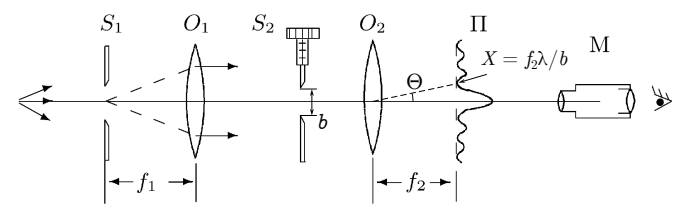
\includegraphics[width=0.83\linewidth]{pics/ustanovka_2}
\caption{Установка 2}
\label{fig:ust-2}
\end{figure}
Дифракционная картина наблюдается в фокальной плоскости объектива $O_2$. Поскольку объектив не вносит дополнительной разности хода между интерферирующими лучами
(\textit{таутохронизм тонкой линзы}), в его фокальной плоскости наблюдается неискажённая
дифракционная картина Фраунгофера, соответствующая бесконечно удалённой плоскости наблюдения.

При дифракции Фраунгофера в центре поля зрения наблюдается дифракционный максимум (светлая полоса). Сбоку от неё наблюдаются чередующиеся минимумы и максимумы с довольно быстро затухающей интенсивностью. Направление на минимумы (тёмныеполосы) при малых углах $\Theta$ определяется соотношением
\begin{equation}
    \Theta^{min}_n = n \frac{\lambda}{b}, \;\; n = \pm1, \pm2, \pm3....
\end{equation}
где $b$ — ширина щели. Каждому значению угла $\Theta$ соответствует точка в плоскости объектива с фокусным расстоянием $f_2$, отстоящая от оптической оси на расстоянии
\begin{equation}
    X_n = f_2 \tg\Theta_n \approx f_2\Theta_n.
\end{equation}

\section*{Задание}
\textbf{1)-3)} Пересобираем систему, добавляя линзу $O_2$, настраиваем микуроскоп на фокальную плоскость линзы П. 

\textbf{4)-5)} Фиксируем значения $f_2 = 138$ мм, $b = (251\pm10)$ мкм и заполняем таблицу значениями. 

\begin{tabular}{|c|c|c|c|}
\hline
$m$  & $X_m$, мм & $b$, мкм & $\Delta b$, мкм \\ \hline
-5 & -1.54    & 259.0 & 1.7      \\ \hline
-4 & -1.32    & 241.7 & 1.8      \\ \hline
-3 & -1.00    & 239.3 & 2.4      \\ \hline
-2 & -0.68    & 234.6 & 3.5      \\ \hline
-1 & -0.31    & 257.3 & 8.3      \\ \hline
1  & 0.31     & 257.3 & 8.3      \\ \hline
2  & 0.68     & 234.6 & 3.5      \\ \hline
3  & 1.00     & 239.3 & 2.4      \\ \hline
4  & 1.32     & 241.7 & 1.8      \\ \hline
5  & 1.54     & 259.0 & 1.7      \\ \hline
\end{tabular}

В данной таблице рассчитываем ширину щели по формуле: $b = \frac{m \lambda f_2}{x_m}$, $\Delta b = b \cdot \mathcal{E}_{X_m}$ сравниваем с тем что измеряем с помощью микрометрического винта. $\overline{b} = 246$ мкм, $\Delta b = 11$ мкм, получается данные из эксперимента совпадают (в пределах погрешности).

\begin{minipage}{0.6\textwidth}
      \begin{tikzpicture}
        \begin{axis}[
          width=1\textwidth,
          height=,
          xlabel={$m$},
          ylabel={$x_m$},
          MyStyle1,
          ]
          \draw[blue, domain=-10:10] plot (\x,0.32090909090909103*\x);
          \addplot[purple, only marks] plot [error bars/.cd,
                x dir=both, x fixed = 0.05,
                y dir=both, y explicit,
                      ] table [
                      x=m, y=x_m,
                x error minus=err, x error plus=err, y error minus=err, y error plus=err, col sep=comma] {x_m(m).csv};
        \end{axis}
      \end{tikzpicture}
\end{minipage}
\begin{minipage}{0.35\textwidth}
    Из графика находим расстояние между соседними максимумами, это просто угол наклона: $\Delta x = (0.321\pm0.005)$ мм. Погрешность находим из формулы взвешенного МНК.
\end{minipage}

\section{Дифракция Фраунгофера на двух щелях}
Схема для наблюдения дифракции Фраунгофера на двух щелях изображена на рис. 3.
По сравнению с рис. 3 в ней щель $S_2$ заменена на экран Э с двумя щелями. При этом щель $S_2$ (с микрометрическим винтом) установлена вместо входной щели $S_1$ (для измерения
влияния ширины источника на чёткость картины).

Результат дифракции на двух щелях можно представить как \textit{интерференцию} дифракционных картин от каждой щели (аналог интерференционной схемы Юнга).
\begin{figure}[h]
\centering
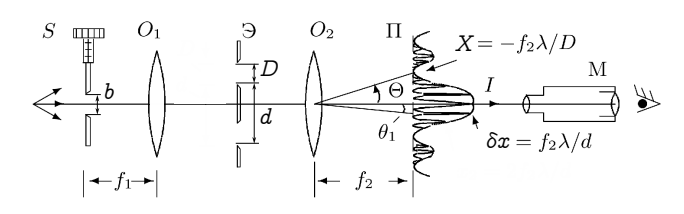
\includegraphics[width=0.83\linewidth]{pics/ustanovka_3}
\caption{Установка 3}
\label{fig:ust-3}
\end{figure}

Если входная щель достаточно узка, то дифракционная картина в плоскости П (рис. 3) подобна той, что получалась при дифракции на одной щели, однако теперь вся картина испещрена рядом дополнительных узких полос. Наличие этих полос объясняется суперпозицией (\textit{интерференцией}) световых волн, приходящих в плоскость наблюдения через разные щели экрана Э. В центре главного дифракционного максимума располагается светлая
полоса (разность на оси, в силу симметрии, равна нулю). Светлая интерференционная полоса наблюдается также, когда разность хода кратна длине волны. Угловая координата $\Theta_n$ интерференционного максимума $n$-го порядка определяется соотношением
\begin{equation}
    \Theta_n d = n \lambda, \;\; n = \pm1, \pm2, \pm3....
\end{equation}
где $d$ — расстояние между щелями. Линейное расстояние $\delta x$ между соседними интерференционными полосами в плоскости П равно поэтому
\begin{equation}
    \delta x = f_2 \frac{\lambda}{d}
\end{equation}
На рис. 4 показано распределение интенсивности в фокальной плоскости объектива $O_2$. Штриховой линией (в увеличенном масштабе) изображено распределение интенсивности при дифракции света на одиночной щели. Поскольку полная угловая ширина главного дифракционного максимума (от минимума до минимума) равна $2\lambda/D$, где $D$ — ширина
отдельной щели, то на нём укладывается
\begin{equation}
    N = \frac{2d}{D}
\end{equation}
\textit{тёмных} интерференционных полос (в центре картины максимум, поэтому светлых полос
— на одну больше). 

При дифракции света на двух щелях чёткая система интерференционных полос наблюдается только при достаточно узкой ширине входной щели ($O_2$), которую можно рассматривать как протяжённый источник света размером $b$. Для наблюдения интерференции необходимо, чтобы расстояние $d$ между щелями не превышало \textit{радиуса когерентности}.
\begin{equation}
    d \leq \rho_{\text{кор}} \approx \frac{\lambda}{b} f_1
\end{equation}
Таким образом, по размытию интерференционной картины можно оценить размер источника $b$. Этот метод используется в звёздном интерферометре при измерении угловых размеров звёзд.

\textbf{} При смещении $S_1$ не происходит сдвига дифракционной картины. 
Это связано с тем, что картина находится в фокальной плоскости 
линзы $S_2$, куда приходят почти параллельные лучи. При уменьшении 
ширины щели картина растягивается, что согласуется с формулой (4).

\section*{Задание}
Получив резкое изображение, определим расстояние между крайними темными полосками внутри центрального максимума и посчитаем число светлых промежутков между ними:\\
$L = (0,720 \pm 0,005)$ мм, между ними $n = 11 \pm 1$ светлых промежутков.\\
Погрешность для $L$ приняли за половину цены деления, а погрешность же для $n$ возьмем равной $1$.\\
Далее определим расстояние $\delta x$ между минимумами по формуле $\delta x = \frac{L}{n} = (65 \pm 5)$ мкм.\\
Тогда из формулы $\delta x = f_2 \frac{\lambda}{d}$ мы можем получить расстояние $d$ между щелями:
\[d = (0,97 \pm 0,05) \text{мм}\]
Где погрешность $d$:
\[\sigma_d = d \cdot \sqrt{\left(\dfrac{\partial \left(f_2 \frac{\lambda}{\delta x}  \right)}{\partial \left(\delta x\right)}\right)^{2} \cdot \sigma_{\delta x}^2} = d \cdot f_2\lambda \dfrac{1}{\delta x^2} \cdot \sigma_{\delta x} = \dfrac{d^2}{\delta x} \sigma_{\delta x}\]
Измерим также $d$ и $D$ (ширину щелей) с помощью микроскопа, получим, что:
\[d = (1,000 \pm 0,005) \text{мм}\]
\[D = (0,180 \pm 0,005) \text{мм}\]
Погрешность берем как половину цены деления.\\
Отсюда из формулы $n = \frac{2d}{D}$ получаем, что:
\[n_{\text{теор}} = 11 \pm 1\]
Погрешность для $n$:
\[\delta n = n \cdot \sqrt{\left(\dfrac{\partial \frac{2d}{D}}{\partial d}\right)^{2} \cdot \delta_{d}^2 + \left(\dfrac{\partial \frac{2d}{D}}{\partial D}\right)^{2} \cdot \delta_{D}^2} = \sqrt{\dfrac{4\delta_d^2}{D^2} + \dfrac{4d^2\delta_{D}^2}{D^4}}\]
Как видно, $n$ и $n_{\text{теор}}$ получились равными.\\
Исследуем также влияние когерентности на видность картины. Для этого, расширяя щель, $S$ подберём $b_0$ такую, при которой первый раз исчезают интерференционные полосы:\\
$b_{0\text{практ}} = (0,0715 \pm 0,0005)$ мм.\\
Из формулы $\dfrac{b}{f_1} = \dfrac{\lambda}{d}$ получаем, что: 
\[b_{0\text{теор}} = (0,060 \pm 0,002) \text{мм}\]
Погрешность для этой формулы опять-таки берется из:
\[\delta b = b \cdot \left|\dfrac{\partial \frac{f_1 \lambda}{d}}{\partial d}\right| \sigma_d = \dfrac{b f_1 \lambda}{d^2} \cdot \sigma_d = \dfrac{b^2\sigma_d}{d}\]
Как видно, $b_{0\text{практ}}$ и $b_{0\text{теор}}$ получились близкими, но все же не равными в пределах доверительных интервалов.
\section{Влияние дифракции на разрешающую способность оптического инструмента}
Поставив между линзами щель $S_2$ и уменьшая ее ширину, пронаблюдаем ухудшение изображения. Подберем ширину $S_2$ так, чтобы изображения почти сливались:
\[D_0 = (0,095 \pm 0,005)\text{мм}\]
Погрешность берем как половину цены деления.\\
Поставим двойную щель и измерим расстояние между щелями и толщину самих щелей: 
\[d = (1,000 \pm 0,005) \text{мм}\]
\[D = (0,180 \pm 0,005) \text{мм}\]
Погрешность берем как половину цены деления.\\
В итоге получаем, что выполнено соотношение:
$\frac{\lambda}{D_0} = 5,87 \cdot 10^{-3} \approx \frac{d}{f_1} = 8,7 \cdot 10^{-3}$.

\section*{Вывод}
В ходе работы было изучено явление дифракции света - дифракция Френеля на щели и на препятствии, дифракция Фраунгофера на одной и двух щелях:
\begin{itemize}
\item При исследовании явления дифракции Френеля на щели убедились, что ширина зон Френеля примерно равна ширине щели.
\item При исследовании явления дифракции Фраунгофера на щели получили значение ширины щели равное в пределах доверительных интервалов измеренному непосредственно с помощью регулятора ширины щели:
\begin{center}
    $b = (223 \pm 0,5) $мкм \hspace{0.5cm} и \hspace{0.5cm} $b = (242,0 \pm 16,7)$ мкм
\end{center}
\item При исследовании явления дифракции Фраунгофера на двух щелях было получено значение расстояния между щелями, примерно равное измеренному с помощью микроскопа:
\begin{center}
    $d = (1,000 \pm 0,005)$ мм \hspace{0.5cm} и \hspace{0.5cm}  $d = (0,97 \pm 0,05)$ мм
\end{center}
\item В ходе изучения влияния дифракции на разрешающую способность оптического инструмента получили, что $D_0 > \lambda f_1/d$, что означает разрешимость изображений по Рэлею, что мы и наблюдали в нашей работе.
\end{itemize}
% \begin{minipage}{0.6\textwidth}
%       \begin{tikzpicture}
%         \begin{axis}[
%           width=1\textwidth,
%           height=,
%           xlabel={$m$},
%           ylabel={$x_m$},
%           MyStyle1,
%           ]
%           \draw[blue, domain=0:100] plot (\x,0.32090909090909103*\x);
%           \addplot[purple, only marks] plot [error bars/.cd,
%                 x dir=both, x fixed = 0.05,
%                 y dir=both, y explicit,
%                       ] table [
%                       x=m, y=1z,
%                 x error minus=merr, x error plus=merr, y error minus=1zerr, y error plus=1zerr, col sep=comma] {m(z^-1).csv};
%         \end{axis}
%       \end{tikzpicture}
% \end{minipage}

\end{document}